\chapter{Gradient Ascent}
\label{cha:gascent}
\section{Konzept}
Unsere Implementation ist eine art von DIRECT encoding. Aber anstelle von lediglich Der Confidenz und einer Klasse, werden die Gradienten mittels einer Kreuz-Entropie zu einer Zielklasse berechnet, welche dann als „orientierungshilfe“ für die weiter manipulation der bilder dienen. -> Das wird als Targeted Backpropagation bezeichnet.


The method keeps the same, whether a random “noisy” image or a “real” image is used initially. Only the modification weights need do be smaller, as the goal is to keep the “original image” as much as recognizable as possible.

\section{Implementierung}
Code modifiziert auf Basis von https://github.com/utkuozbulak/pytorch-cnn-adversarial-attacks


Training und Evaluierung des AlexNet Modells

Quelle Des AlexNet hinzufügen.
https://papers.nips.cc/paper/4824-imagenet-classification-with-deep-convolutional-neural-networks.pdf

WICHTIG, aber eigentlich ist können wir das genauso wichtig behandeln wie die Aphrodite?
Unterschied zur Aphrodite? Eigenes modell vs Alexnet architektur die auf die 43-Klassen angepasst wurde. 
Training und Evaluierung des AlexNet mit dem GTSRB Datensatz

Abschluss des Training mit genauigkeit von 89%


Bilderzeugung anhand des Gradient Ascent Fooling Verfahrens REF NGUYEN

WICHTIG
Anwendung des Gradient Ascent Fooling Verfahrens auf das trainierte AlexNet


Generierung eines zufallsbildes (random noise)
iterativer ablauf: 
prediction
gradienten berechnung durch kreuzentropie zur gewünschten klasse
modifikation des bildes durch anteil der gradienten 

Der vorgestellte ansatz ändert sich nicht bei eingabe eines ausgewählten Bildes, die veränderungsrate solle aber gering gehalten werden, um das bild so wenig wie nötig zu verändern

\section{Ergebnisse}
43 bilder Erzeugt respektive 1 pro vorhandene Klasse (im GTSRB Datensatz)
20 Bilder für mit 10 verschiednen klassen erreichten konfidenz höher 0.9

\begin{tabular}{cc}
	\centering
	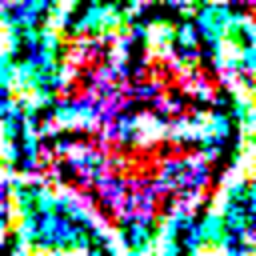
\includegraphics[width=.23\linewidth]{Images/AnPe/17_Einfahrtverbot} &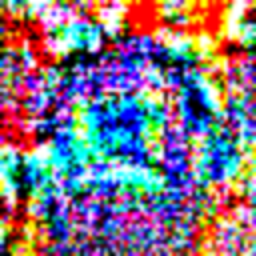
\includegraphics[width=.23\linewidth]{Images/AnPe/34_kreisverkehr_origTurnleft}  \\
	Einfahrt Verboten & Kreisverkehr \\
	& (Ursprünglich als Links abbiegen erzeugt)\\
	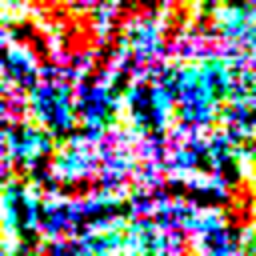
\includegraphics[width=.23\linewidth]{Images/AnPe/39_RechtsVorbeiOrigLinksvorbei} &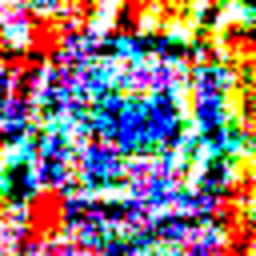
\includegraphics[width=.23\linewidth]{Images/AnPe/40_kreisverkehr}  \\
	Rechts Vorbei& Kreisverkehr\\
\end{tabular}